% The two routes through the library, as the five steps of usage.tex,
% section "Using a scheme, step by step": one decision on the shape of the
% state, then the plain-array route (left) or the model-class route (right),
% row by row the same steps, joined again at step 5, the same call on both.
\documentclass[tikz,border=6pt]{standalone}
\usepackage{amsmath}
\usetikzlibrary{positioning,fit,arrows.meta,calc,backgrounds,shapes.geometric}

% Palette: operations grey, the decision and the shared results blue, route bands light grey.
\definecolor{opcol}{RGB}{235,235,235}
\definecolor{keycol}{RGB}{214,230,245}
\definecolor{bandcol}{RGB}{247,247,247}
\newcommand{\code}[1]{{\footnotesize\texttt{#1}}}

\begin{document}
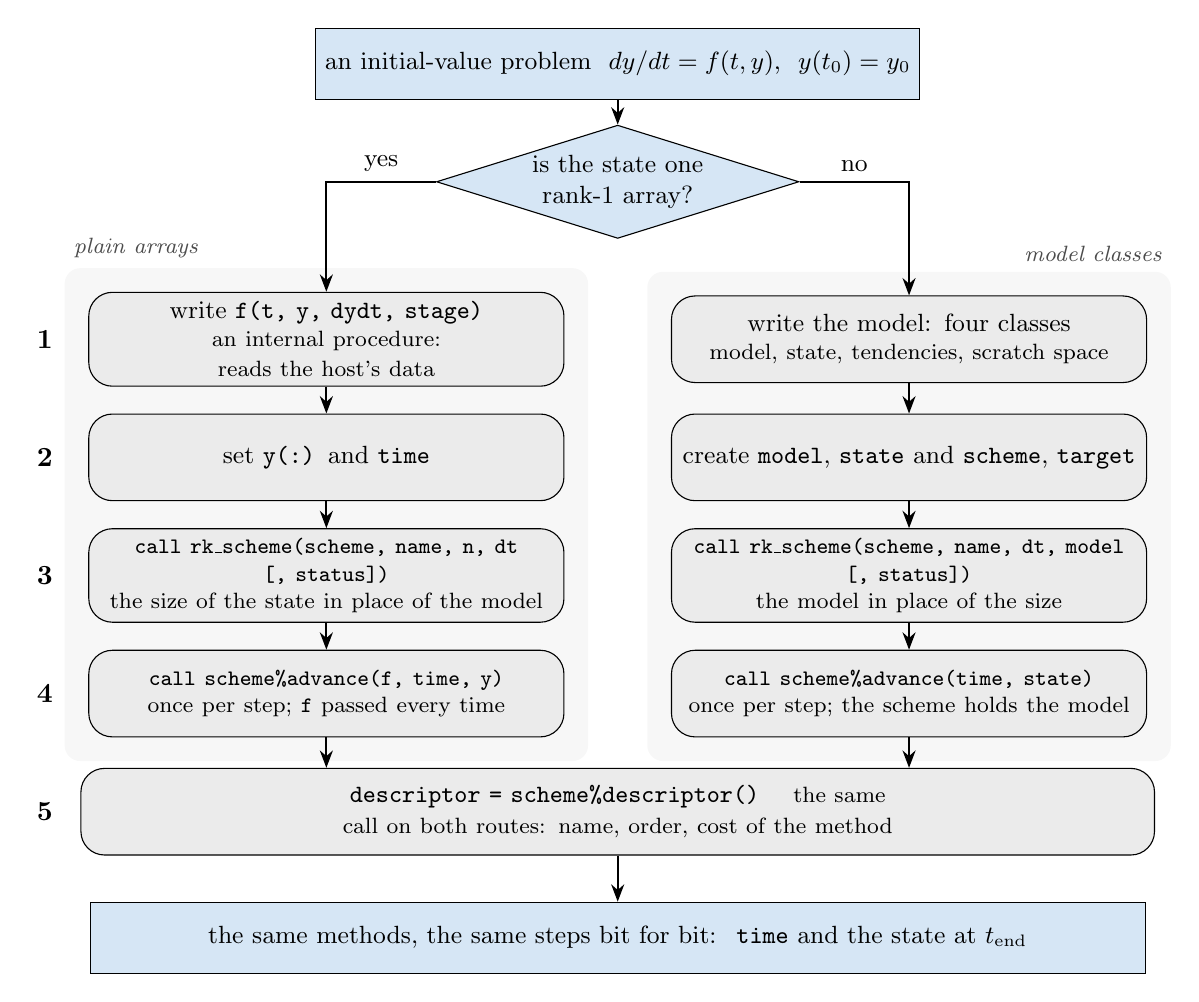
\begin{tikzpicture}[
    font=\small,
    >={Stealth[length=2.2mm]},
    op/.style={draw, rounded corners=3mm, fill=opcol, minimum height=11mm,
               text width=58mm, align=center},                                    % one step of a route
    key/.style={draw, fill=keycol, minimum height=9mm, align=center},              % where the routes meet
    choice/.style={draw, diamond, aspect=3.2, fill=keycol, align=center,
                   inner sep=1pt},                                                 % the one decision
    flow/.style={->, thick},                                                       % the order of the steps
    steplabel/.style={font=\bfseries, anchor=east},                                     % row label: the step number
    note/.style={font=\footnotesize\itshape, text=black!70, align=center},         % explanatory note
  ]

  % ---- grid: left route at x = 0, right route at x = 7.4, one row per step ----
  \def\xL{0}
  \def\xR{7.4}
  \def\yQ{1.6}       % row of the decision
  \def\yA{-0.4}      % 1. the right-hand side / the model
  \def\yB{-1.9}      % 2. the initial condition
  \def\yC{-3.4}      % 3. the scheme
  \def\yD{-4.9}      % 4. the time loop
  \def\yE{-6.4}      % 5. what was run
  \def\yF{-8.0}      % the results, shared

  % ---- the decision ----
  \node[key, minimum width=60mm] (problem) at ({(\xL+\xR)/2}, {\yQ+1.5})
       {an initial-value problem \ $dy/dt = f(t, y)$, \ $y(t_0) = y_0$};
  \node[choice] (q) at ({(\xL+\xR)/2}, \yQ) {is the state one\\rank-1 array?};
  \draw[flow] (problem) -- (q);

  % ---- left route: plain arrays ----
  \node[op] (a1) at (\xL, \yA) {write \texttt{f(t, y, dydt, stage)}\\[-1pt]
                                {\footnotesize an internal procedure: reads the host's data}};
  \node[op] (a2) at (\xL, \yB) {set \texttt{y(:)} and \texttt{time}};
  \node[op] (a3) at (\xL, \yC) {\code{call rk\_scheme(scheme, name, n, dt}\\[-1pt]
                                \code{[, status])}\\[-1pt]
                                {\footnotesize the size of the state in place of the model}};
  \node[op] (a4) at (\xL, \yD) {\code{call scheme\%advance(f, time, y)}\\[-1pt]
                                {\footnotesize once per step; \texttt{f} passed every time}};

  % ---- right route: model classes ----
  \node[op] (b1) at (\xR, \yA) {write the model: four classes\\[-1pt]
                                {\footnotesize model, state, tendencies, scratch space}};
  \node[op] (b2) at (\xR, \yB) {create \texttt{model}, \texttt{state} and \texttt{scheme}, \texttt{target}};
  \node[op] (b3) at (\xR, \yC) {\code{call rk\_scheme(scheme, name, dt, model}\\[-1pt]
                                \code{[, status])}\\[-1pt]
                                {\footnotesize the model in place of the size}};
  \node[op] (b4) at (\xR, \yD) {\code{call scheme\%advance(time, state)}\\[-1pt]
                                {\footnotesize once per step; the scheme holds the model}};

  % ---- step 5, the same call on both routes ----
  \node[op, text width=134mm] (m5) at ({(\xL+\xR)/2}, \yE) {\texttt{descriptor = scheme\%descriptor()} \quad
       {\footnotesize the same call on both routes: name, order, cost of the method}};

  % ---- the branches ----
  \draw[flow] (q.west) -| node[pos=0.25, above] {yes} (a1.north);
  \draw[flow] (q.east) -| node[pos=0.25, above] {no} (b1.north);
  \foreach \r in {a, b} {
    \draw[flow] (\r1) -- (\r2);
    \draw[flow] (\r2) -- (\r3);
    \draw[flow] (\r3) -- (\r4);
    \draw[flow] (\r4.south) -- (\r4.south |- m5.north);
  }

  % ---- where the routes meet ----
  \node[key, minimum width=134mm] (out) at ({(\xL+\xR)/2}, \yF)
       {the same methods, the same steps bit for bit: \ \texttt{time} and the state at $t_{\mathrm{end}}$};
  \draw[flow] (m5) -- (out);

  % ---- row labels: the five steps ----
  \foreach \y/\n in {\yA/1, \yB/2, \yC/3, \yD/4, \yE/5} {
    \node[steplabel] at ({\xL-3.35}, \y) {\n};
  }

  % ---- route bands, behind ----
  \begin{scope}[on background layer]
    \node[fill=bandcol, rounded corners=2mm, inner sep=3mm, fit=(a1)(a4),
          label={[note, anchor=south west]north west:plain arrays}] (bandA) {};
    \node[fill=bandcol, rounded corners=2mm, inner sep=3mm, fit=(b1)(b4),
          label={[note, anchor=south east]north east:model classes}] (bandB) {};
  \end{scope}
\end{tikzpicture}
\end{document}
